\documentclass[a4paper,% DIN A4-Papier
			12pt, 		% 12er Schrift
			DIV=calc, 	% Seitenränder optimieren
			oneside, 	% einseitiges "Buch"
			headsepline, 	% Trennlinie unter dem Seitenkopf
			ngerman, 	% deutscher Text
			smallheadings, 	% kleinere Überschriften 
			openany, 	% neue Kapitel fangen auf einer neuen freien Seite an
			liststotoc, 	% Verzeichnisse kommen ins Inhaltsverzeichnis
			bibtotoc]	% Literaturverzeichnis kommt ins Inhaltsverzeichnis
			{scrbook} 	% KOMA-Klasse "Buch"
%%%%%%%%%%%%%%%%%%%%%%%%%%%%%%%%%%%%%%%
\input{/home/produnis/Dokumente/LaTeX/src/produnis-src-en}		% alle meine LaTeX-Befehle
\usepackage{bbding}
%\usepackage[numbers,round]{natbib}
\setlength{\parindent}{0mm}

%
\pdfinfo{/Title FreeQDA - Manual}  % PDF-Info
%
%%%%%%%%%%%%%%%%%%%%%%%%%%%%%%%%%%%%%%%%
%%%%%%%%%%%%%%%%%%%%%%%%%%%%%%%%%%%%%%%%
\begin{document}
\input{/home/produnis/Dokumente/LaTeX/src/mintedSRC}
\bibliographystyle{/home/produnis/Dokumente/LaTeX/src/bmc_article}	% verwendet den natbib-Literaturstyle
%\bibliographystyle{alphadin}

\shorthandoff{"}			% aus "A wird NICHT Ä!
	
%%%%%%%%%%%%%%%%%%%%%%  D E C K B L A T T
%================================================
\begin{titlepage}

\begin{center}


% Upper part of the page
\textsc{\LARGE FreeQDA}\\[1.5cm]
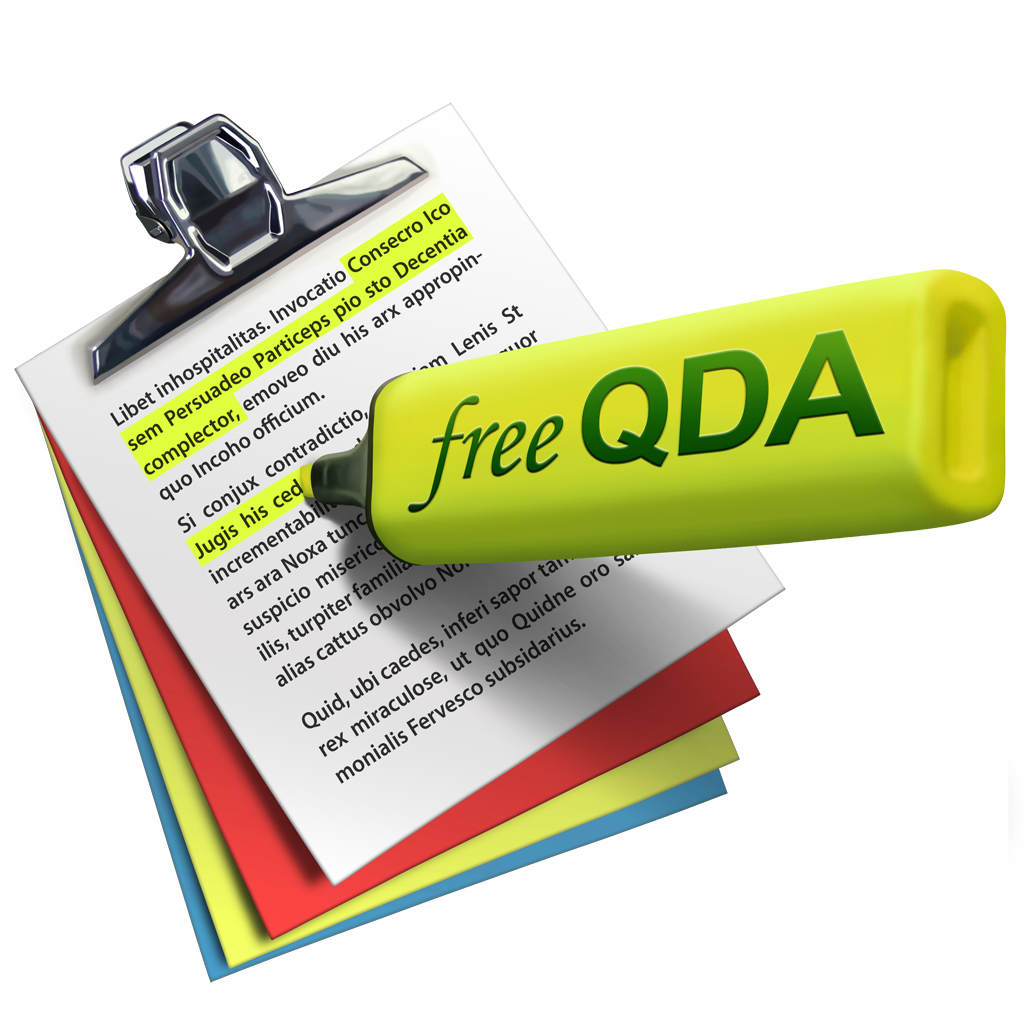
\includegraphics[width=0.25\textwidth]{img/freeQDA_FINAL_1024}\\[1cm]    



\textsc{\Large A free tool for analysis of \\qualitative research data}\\[0.5cm]


% Title
\HRule \\[0.4cm]
{ \huge \bfseries English Manual}\\[0.4cm]

\HRule \\[1.5cm]

% Author and supervisor
\begin{minipage}{0.4\textwidth}
\begin{flushleft} \large
\emph{Author:}\\
Jörg \textsc{große Schlarmann}
\end{flushleft}
\end{minipage}
\begin{minipage}{0.4\textwidth}
\begin{flushright} \large
\emph{and} \\
Dirk \textsc{Kitscha}
\end{flushright}
\end{minipage}

\vfill

% Bottom of the page
{\large \today}

\end{center}

\end{titlepage}

%%%%%%%%%%%%%%  V O R S P A N N
%------------------------------------------------------------
\frontmatter  % dies leitet einführende Seiten ein. Die Seitenzahlen werden römisch angezeigt
\section*{About}
FreeQDA is a free and open source software project for the analysis of qualitative research data.

FreeQDA is published under the terms of the GPLv2.

The initial development of FreeQDA was funded by the \emph{German Society of Nursing Science}\footnote{\url{http://www.dg-pflegewissenschaft.de}} %
(Deutsche Gesellschaft für Pflegewissenschaft DGP)
%----
\tableofcontents	% Inhaltsverzeichnis ausgeben

%%%%%%%%%%%%%% H A U P T T E I L
%-----------------------------------------------------------
\mainmatter   % dies leitet den Haupttext ein. Die Seitenzahlen werden arabisch angezeigt
\include{include/en-start}
%\include{include/20schliessend}
%
%
%
%-------------------------------------------------------------------
\bibliography{freeqda_manual}
\listoffigures		% beginnend mit dem Abbildungsverzeichnis
\listoftables		%... und dem Tabellenverzeichnis
\listoflistings		% aus dem minted-Paket
\newpage
\printnomenclature	% Abkürzungsverzeichnis ausgeben
%-------------------------
\backmatter    % hiermit wird  der Nachspann eingeleitet. Seitenzahlen werden weiter fortgeführt
\appendix
\addcontentsline{toc}{chapter}{Anhang}
% \input{includes/Linkliste}
%\theendnotes
%
%---------------------
\end{document}
%%%%%%%%%%%%%%%%%%%%%%%%%%%%%%%%%%%%%%%%
%%%%%%%%%%%%%%%%%%%%%%%%%%%%%%%%%%%%%%%%
%%%%%%%%%%%%%%%%%%%%%%%%%%%%%%%%%%%%%%%%
%
%%%%% end of file